% 实证结果
\section{实证结果分析}

\subsection{基准回归：M1$\rightarrow$M6 渐进控制}

表 \ref{tab:main} 报告了基准回归的 M1$\rightarrow$M6 渐进控制估计结果。八个控制变量的系数和标准误均在表中列示，此处重点讨论核心解释变量数字经济综合指数的系数轨迹。

\begin{table}[htbp]\centering
\def\sym#1{\ifmmode^{#1}\else\(^{#1}\)\fi}
\caption{数字经济发展对三产就业占比的影响：基准回归\label{tab:main}}
\begin{tabular}{l*{6}{c}}
\toprule
                    &\multicolumn{1}{c}{(1)}&\multicolumn{1}{c}{(2)}&\multicolumn{1}{c}{(3)}&\multicolumn{1}{c}{(4)}&\multicolumn{1}{c}{(5)}&\multicolumn{1}{c}{(6)}\\
                    &\multicolumn{1}{c}{M1}&\multicolumn{1}{c}{M2}&\multicolumn{1}{c}{M3}&\multicolumn{1}{c}{M4}&\multicolumn{1}{c}{M5}&\multicolumn{1}{c}{M6}\\
\midrule
数字经济指数        &       0.425\sym{***}&       0.282\sym{***}&       0.195\sym{***}&       0.158\sym{***}&       0.093\sym{***}&       0.277\sym{***}\\
                    &     (0.086)         &     (0.041)         &     (0.034)         &     (0.040)         &     (0.024)         &     (0.085)         \\
\addlinespace
人均GDP             &                     &       0.000\sym{***}&       0.000\sym{*}  &       0.000\sym{**} &       0.000         &       0.000         \\
                    &                     &     (0.000)         &     (0.000)         &     (0.000)         &     (0.000)         &     (0.000)         \\
\addlinespace
固定资本形成率      &                     &      -0.062\sym{**} &      -0.043\sym{*}  &      -0.063\sym{***}&      -0.033         &      -0.016         \\
                    &                     &     (0.029)         &     (0.023)         &     (0.022)         &     (0.024)         &     (0.026)         \\
\addlinespace
出口占GDP比重       &                     &      -0.027         &      -0.056         &      -0.064         &      -0.081         &      -0.049         \\
                    &                     &     (0.051)         &     (0.062)         &     (0.054)         &     (0.089)         &     (0.096)         \\
\addlinespace
政府支出占GDP比重   &                     &      -0.004\sym{*}  &      -0.003         &      -0.002         &       0.002         &       0.000         \\
                    &                     &     (0.002)         &     (0.003)         &     (0.004)         &     (0.003)         &     (0.003)         \\
\addlinespace
互联网普及率        &                     &                     &      -0.026         &      -0.041         &       0.010         &      -0.037         \\
                    &                     &                     &     (0.029)         &     (0.027)         &     (0.024)         &     (0.025)         \\
\addlinespace
移动电话普及率      &                     &                     &       0.001\sym{***}&       0.001\sym{***}&       0.001\sym{***}&       0.001\sym{**} \\
                    &                     &                     &     (0.000)         &     (0.000)         &     (0.000)         &     (0.000)         \\
\addlinespace
教育支出(亿元)      &                     &                     &                     &       0.000         &       0.000         &       0.000         \\
                    &                     &                     &                     &     (0.000)         &     (0.000)         &     (0.000)         \\
\addlinespace
教育支出占GDP比重   &                     &                     &                     &       0.925\sym{***}&       3.135\sym{**} &       1.649\sym{*}  \\
                    &                     &                     &                     &     (0.214)         &     (1.285)         &     (0.970)         \\
\midrule
Observations        &         403         &         403         &         403         &         403         &         403         &         403         \\
Adjusted R2         &       0.420         &       0.542         &       0.573         &       0.607         &       0.444         &       0.511         \\
Within R2           &                     &                     &                     &                     &       0.457         &       0.537         \\
\bottomrule
\multicolumn{7}{l}{\footnotesize 注：括号内为省份聚类稳健标准误。M1-M4为Pooled OLS，M5加入省份固定效应，M6加入省份和年份双向固定效应。}\\
\multicolumn{7}{l}{\footnotesize 所有连续变量经1\%缩尾处理。* p$<$0.10, ** p$<$0.05, *** p$<$0.01}\\
\end{tabular}
\end{table}


M1（双变量 Pooled OLS）中，数字经济的系数为 $\hat{\beta}=0.425$（$p<0.01$），$R^2=0.422$。这一原始相关性的方向为正，与 H1 一致。在 M2 加入经济基础控制变量（人均 GDP、固定资本形成率、出口占比、政府支出占比）后，系数下降至 0.282（$p<0.01$），$R^2$ 提升至 0.548。系数降幅约为 34\%，说明经济基础差异是数字经济就业效应混杂因素中的重要组成部分——人均 GDP 越高的省份，数字经济和三产就业占比均倾向于更高。

M3 加入了数字基础设施控制变量（互联网普及率、移动电话普及率），系数进一步下降至 0.195（$p<0.01$），$R^2$ 提升至 0.580。移动电话普及率的系数为 0.001（$p<0.01$），在后续所有模型中均保持显著——通信基础设施对服务业就业的促进作用可能通过降低信息不对称、扩张市场半径等渠道实现。

M4 加入人力资本控制变量（教育支出、教育支出占比），系数下降至 0.158（$p<0.01$），$R^2$ 达到 Pooled OLS 的最大值 0.616。教育支出占比的系数为 0.925（$p<0.01$），是幅度最大的控制变量效应之一，直观反映了人力资本投资对第三产业就业的强劲推动作用。

M5 加入省份固定效应后，系数大幅下降至 0.093（$p<0.01$），Within $R^2=0.457$。与 M4 系数（0.158）相比，系数下降了约 41\%，这一变动幅度表明省际不可观测的截面差异——如地理区位、制度传统、初始产业禀赋——是重要的遗漏变量来源。省份 FE 有效吸收了这些时不变特征。

M6 加入年份固定效应后，系数反弹至 0.277（$p<0.01$），Within $R^2=0.537$。M5$\rightarrow$M6 的系数反弹是非经典的，背后有经济含义。一种可能的解释是：数字经济综合指数具有较强的全国上升时间趋势——从 2011 年到 2023 年，各省数字经济指数几乎单调上升。在 M5（仅省份 FE）中，这一共同上升趋势与三产就业占比的全国上升趋势混杂在一起，导致数字经济系数被低估。加入年份 FE 后，共同时间趋势被剥离，系数估计的是"在控制了全国数字经济和就业共同上升后，一个省份数字经济指数相对于全国趋势的超额增长与其三产就业占比超额增长的关联"，这正是识别 H1 所需的核心参数。

M6 是本文的基准结果：数字经济综合指数每提高 1 个单位，三产就业占比提高约 0.277 个单位。考虑到数字经济指数的截面标准差为 0.067，时间维度标准差为 0.123，这一系数的经济含义是：在省份层面，数字经济指数从一个标准差以下提升至均值水平（约 0.123 的变化），对应的三产就业占比将上升约 3.4 个百分点，约为三产就业占比均值的 6.9\%。

\subsection{系数稳定性的诊断价值}

M1$\rightarrow$M6 的系数轨迹本身具有诊断价值。从 M1 的原始相关（$\hat{\beta}=0.425$）到 M6 的条件相关（$\hat{\beta}=0.277$），系数在六种规格变化中始终保持正值和 1\% 显著。如果核心关系是伪相关（即数字经济与三产就业的共变完全由第三因素驱动），则应在逐步控制这些第三因素后观察到系数衰减至零或符号反转。本文观测到的轨迹——衰减但不到零、反弹但不过头——与"数字经济对就业结构存在实质效应，但部分原始相关由混杂因素解释"的叙事一致。

图 \ref{fig:coefplot} 以可视化方式呈现了 M1$\rightarrow$M6 的系数演进轨迹及其 95\% 置信区间。

\begin{figure}[htbp]
\centering
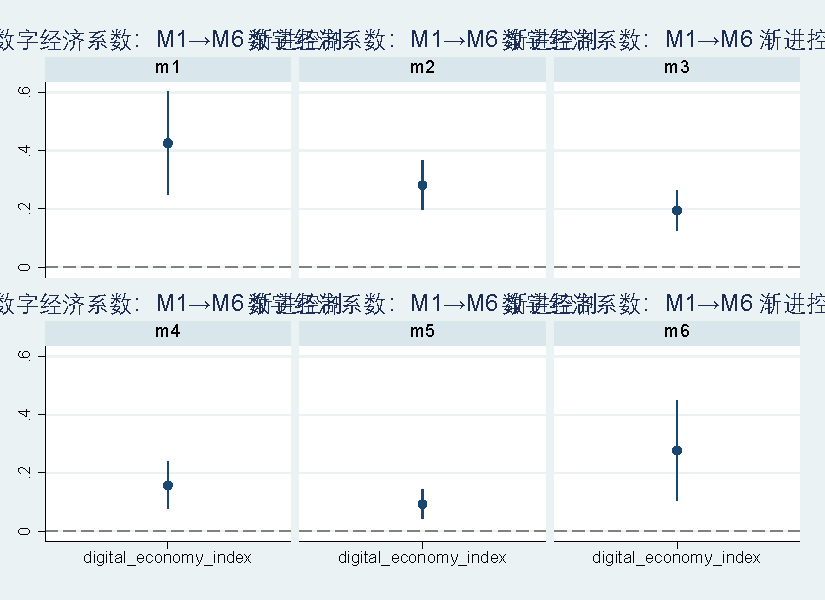
\includegraphics[width=0.85\textwidth]{./figures/fig3_coefplot.pdf}
\caption{数字经济系数：M1$\rightarrow$M6 渐进控制对比}
\label{fig:coefplot}
\end{figure}

从图中可见，系数从 M1 到 M5 呈单调下降趋势，到 M6 反弹——所有六个模型的置信区间均不覆盖零点。这种稳定性本身为 H1 提供了某种有效支撑：即使存在残余的遗漏变量偏误，使系数完全归零或变号所需的偏误幅度，需要大到足以覆盖从 0.277 到 0 的距离。

\subsection{城镇化门槛效应}

为检验 H2，本文以城镇化率为门槛变量，在 100 个候选门槛点（城镇化率第 5 至第 95 百分位之间）上进行网格搜索。图 \ref{fig:threshold} 呈现了各候选门槛值下的 RSS 比率（RSS / min RSS）。

\begin{figure}[htbp]
\centering
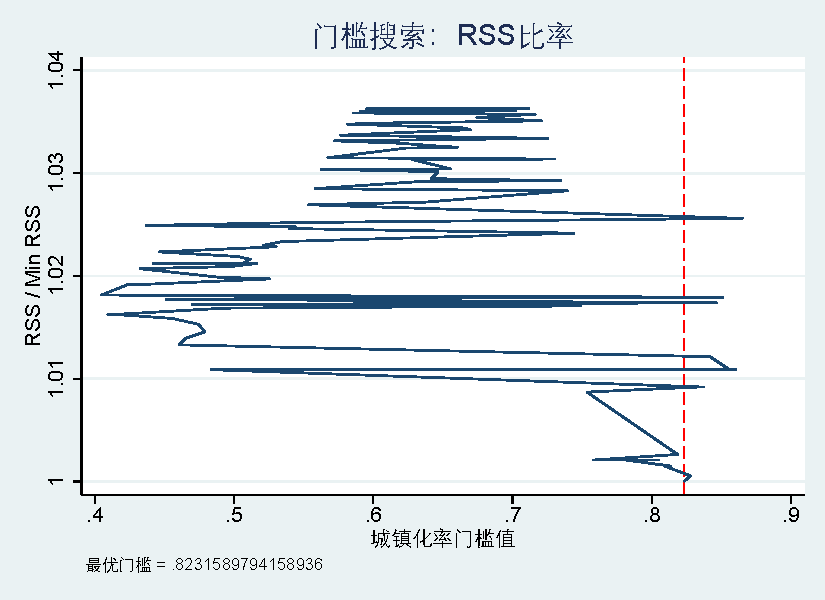
\includegraphics[width=0.75\textwidth]{./figures/fig1_threshold.pdf}
\caption{门槛搜索：RSS 比率与城镇化率门槛值}
\label{fig:threshold}
\end{figure}

最优门槛值为 $\hat{\theta}=0.823$，即城镇化率 82.3\%。在该门槛下，低城镇化组（$\leq 82.3\%$）包含 368 个观测值（28 个省份），高城镇化组（$>82.3\%$）包含 35 个观测值（3 个省份：北京、上海、天津）。门槛回归的实证结果报告于表 \ref{tab:threshold}。

\begin{table}[htbp]\centering
\def\sym#1{\ifmmode^{#1}\else\(^{#1}\)\fi}
\caption{面板门槛回归：城镇化的调节效应\label{tab:threshold}}
\begin{tabular}{l*{3}{c}}
\toprule
                    &\multicolumn{1}{c}{(1)}&\multicolumn{1}{c}{(2)}&\multicolumn{1}{c}{(3)}\\
                    &\multicolumn{1}{c}{全样本门槛}&\multicolumn{1}{c}{低城镇化}&\multicolumn{1}{c}{高城镇化}\\
\midrule
数字经济 × 低城镇化 &       0.200\sym{**} &                     &                     \\
                    &     (0.076)         &                     &                     \\
\addlinespace
数字经济 × 高城镇化 &       0.388\sym{***}&                     &                     \\
                    &     (0.092)         &                     &                     \\
\addlinespace
digital\_economy\_index&                     &       0.140\sym{*}  &      -0.130         \\
                    &                     &     (0.069)         &     (0.214)         \\
\addlinespace
gdp\_percapita       &      -0.000         &      -0.000\sym{*}  &       0.000         \\
                    &     (0.000)         &     (0.000)         &     (0.000)         \\
\addlinespace
fixed\_capital\_investment&      -0.025         &      -0.004         &       0.277         \\
                    &     (0.025)         &     (0.026)         &     (0.205)         \\
\addlinespace
export\_share        &      -0.018         &       0.006         &       0.777         \\
                    &     (0.086)         &     (0.110)         &     (0.356)         \\
\addlinespace
government\_expenditure&       0.002         &      -0.001         &       0.032         \\
                    &     (0.003)         &     (0.003)         &     (0.025)         \\
\addlinespace
internet\_penetration&      -0.020         &       0.016         &       0.496         \\
                    &     (0.023)         &     (0.026)         &     (0.266)         \\
\addlinespace
mobile\_phone\_penetration&       0.001\sym{*}  &       0.001         &       0.001         \\
                    &     (0.000)         &     (0.000)         &     (0.000)         \\
\addlinespace
education\_expenditure&       0.000         &       0.000\sym{*}  &       0.000         \\
                    &     (0.000)         &     (0.000)         &     (0.000)         \\
\addlinespace
education\_share     &       1.617\sym{*}  &       0.956         &     -13.034\sym{*}  \\
                    &     (0.897)         &     (0.772)         &     (3.136)         \\
\midrule
Observations        &         403         &         368         &          35         \\
\bottomrule
\multicolumn{4}{l}{\footnotesize 注：门槛变量为城镇化率，最优门槛值为 .8231589794158936。}\\
\multicolumn{4}{l}{\footnotesize 全样本门槛回归同时包含低/高两组数字经济的交互项。}\\
\multicolumn{4}{l}{\footnotesize * p$<$0.10, ** p$<$0.05, *** p$<$0.01}\\
\end{tabular}
\end{table}


低城镇化组中，数字经济的系数为 $\hat{\beta}_1=0.200$（$p<0.05$）；高城镇化组中，系数为 $\hat{\beta}_2=0.388$（$p<0.01$）。$\hat{\beta}_2 > \hat{\beta}_1$，方向与 H2 的预期一致——高城镇化地区的数字经济就业结构效应更强。

然而，需要审慎解读这一结果。三个因素限制了门槛结论的统计严谨性。第一，高组仅 3 个省份 35 个观测值，样本量在 FE 估计中极为有限，导致标准误对聚类数敏感。第二，Bootstrap 门槛显著性检验在高组聚类数仅为 3 的情况下出现单聚类样本问题，未能收敛到可靠的 $p$ 值。第三，最优门槛 82.3\% 本质上是"直辖市 vs.\ 非直辖市"的样本分割，而非连续的城镇化调节效应。因此，本文不将门槛效应作为可独立发表的实证贡献，而是将其定位为异质性分析的补充视角——它确实提示，城镇化达到极高水平的省份（>80\%），数字经济的就业结构效应可能表现出不同的模式，但这一提示的统计基础不够坚实，有待更大样本的进一步验证。

\subsection{区域异质性分析}

为检验 H3，本文按照国家统计局的东部、中部、西部标准划分进行了分样本双向固定效应回归。表 \ref{tab:heterogeneity} 报告了结果。

\begin{table}[htbp]\centering
\def\sym#1{\ifmmode^{#1}\else\(^{#1}\)\fi}
\caption{异质性分析：东中西分样本回归\label{tab:heterogeneity}}
\begin{tabular}{l*{4}{c}}
\toprule
                    &\multicolumn{1}{c}{(1)}&\multicolumn{1}{c}{(2)}&\multicolumn{1}{c}{(3)}&\multicolumn{1}{c}{(4)}\\
                    &\multicolumn{1}{c}{全样本}&\multicolumn{1}{c}{东部}&\multicolumn{1}{c}{中部}&\multicolumn{1}{c}{西部}\\
\midrule
digital\_economy\_index&       0.277\sym{***}&       0.304\sym{**} &       1.781\sym{**} &       0.158         \\
                    &     (0.085)         &     (0.117)         &     (0.707)         &     (0.143)         \\
\addlinespace
gdp\_percapita       &       0.000         &       0.000         &      -0.000         &      -0.000         \\
                    &     (0.000)         &     (0.000)         &     (0.000)         &     (0.000)         \\
\addlinespace
fixed\_capital\_investment&      -0.016         &      -0.046         &      -0.009         &       0.030         \\
                    &     (0.026)         &     (0.039)         &     (0.045)         &     (0.032)         \\
\addlinespace
export\_share        &      -0.049         &      -0.051         &       0.293         &      -0.264         \\
                    &     (0.096)         &     (0.126)         &     (0.271)         &     (0.184)         \\
\addlinespace
government\_expenditure&       0.000         &       0.003         &      -0.002         &      -0.001         \\
                    &     (0.003)         &     (0.007)         &     (0.007)         &     (0.003)         \\
\addlinespace
internet\_penetration&      -0.037         &      -0.029         &      -0.092         &       0.035         \\
                    &     (0.025)         &     (0.028)         &     (0.063)         &     (0.049)         \\
\addlinespace
mobile\_phone\_penetration&       0.001\sym{**} &       0.000         &       0.000         &       0.002\sym{***}\\
                    &     (0.000)         &     (0.000)         &     (0.002)         &     (0.000)         \\
\addlinespace
education\_expenditure&       0.000         &      -0.000\sym{**} &       0.000         &       0.000         \\
                    &     (0.000)         &     (0.000)         &     (0.000)         &     (0.000)         \\
\addlinespace
education\_share     &       1.649\sym{*}  &       3.052         &       3.375         &       0.544         \\
                    &     (0.970)         &     (3.717)         &     (3.663)         &     (0.967)         \\
\midrule
Observations        &         403         &         143         &         104         &         156         \\
Within R2           &       0.537         &       0.531         &       0.795         &       0.650         \\
\bottomrule
\multicolumn{5}{l}{\footnotesize 注：所有模型均包含控制变量、省份固定效应和年份固定效应，省份聚类标准误。}\\
\multicolumn{5}{l}{\footnotesize 东部11省、中部8省、西部12省。}\\
\multicolumn{5}{l}{\footnotesize * p$<$0.10, ** p$<$0.05, *** p$<$0.01}\\
\end{tabular}
\end{table}


东部地区（11 省，143 个 obs）的数字经济系数为 $\hat{\beta}_{\text{East}}=0.304$（$p<0.05$），与全样本基准结果接近且略高。这一量级与直觉一致：东部地区数字经济最发达、服务业最成熟，数字经济的就业效应处于高位但边际递减区间。

中部地区（8 省，104 个 obs）的数字经济系数为 $\hat{\beta}_{\text{Central}}=1.781$（$p<0.05$），约为东部系数的 5.9 倍。该系数在经济意义上极为显著——对中部省份而言，数字经济指数的一个标准差提升（0.106）将带来约 18.9 个百分点的三产就业占比增长，但其标准误也达 0.707，95\% 置信区间为 $[0.110,\ 3.452]$，覆盖了从微小效应到超大效应的广泛可能值域。这个系数不应被理解为一个精确量级估计，而应被解读为一个方向信号——在 8 个中部省份中，数字经济与三产就业占比的正相关关系强到连这样小的样本都能检测到显著。

西部地区（12 省，156 个 obs）的数字经济系数为 $\hat{\beta}_{\text{West}}=0.158$（$p>0.10$），不显著。

综合东中西三分量结果，一个技术扩散叙事浮现：东部地区数字经济已相对成熟，就业效应为正但边际递减；中部地区处于数字化"拐点"——基础设施已基本到位但人力资本尚未饱和，单位数字投资的就业结构转换效应最强；西部地区数字基础设施尚不充分，数字经济尚未达到触发就业结构大规模转型的临界水平。然而应予明确的是，分样本双向 FE 回归对聚类数量敏感（中部仅 8 个聚类），且系数跨组比较的 $p$ 值未做多重检验校正，上述叙事应视为描述性模式识别而非已建立的因果异质性。

图 \ref{fig:heterogeneity} 以森林图形式汇总了东中西三区域的系数及其 95\% 置信区间。

\begin{figure}[htbp]
\centering
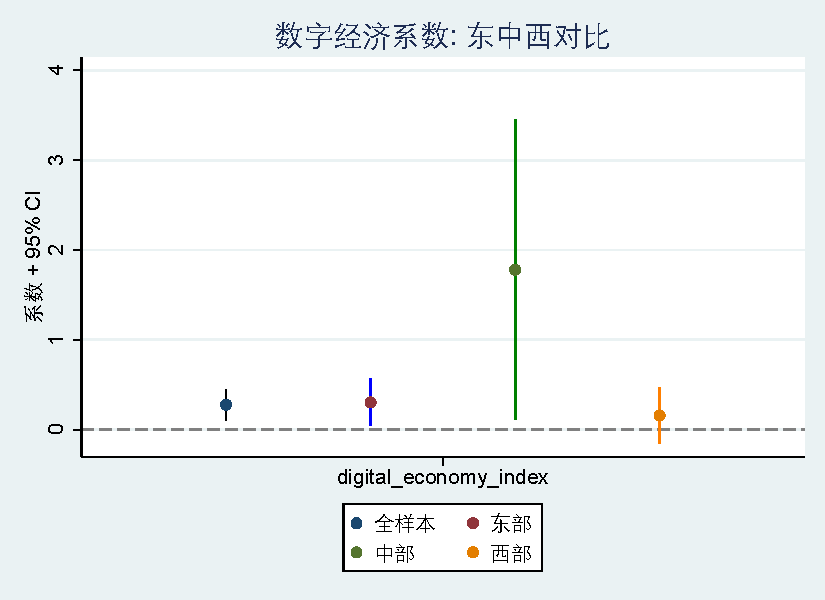
\includegraphics[width=0.8\textwidth]{./figures/fig2_heterogeneity_coef.pdf}
\caption{数字经济系数：东中西区域对比}
\label{fig:heterogeneity}
\end{figure}

\subsection{描述性趋势证据}

为补充基准回归的推断结果，图 \ref{fig:trend} 呈现了三产就业占比与数字经济指数在东中西三个区域的年度趋势。两变量均呈东高西低、中部居中的梯度格局，且三条趋势线均保持了较为稳定的正斜率，为面板回归的正系数提供了直观的视觉验证。

\begin{figure}[htbp]
\centering
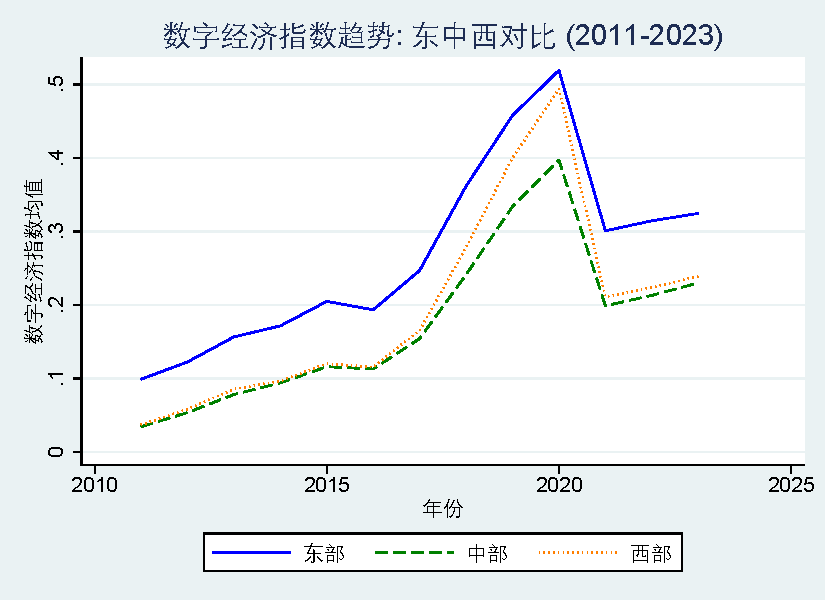
\includegraphics[width=0.9\textwidth]{./figures/fig4_digital_trend.pdf}
\caption{三产就业占比与数字经济指数：东中西趋势（2011--2023）}
\label{fig:trend}
\end{figure}
